\chapter{Magnesium-24 ($^{24}_{12}\text{Mg}$): The Six-Alpha Octahedron}
\label{ch:magnesium}

\begin{objectivebox}
\begin{itemize}
    \item Model Magnesium-24 as the $6\alpha$ octahedral shell closure.
    \item Track the systematic $V_R/V_{BR}$ escalation from $0.019$ (Carbon) to $0.040$ (Magnesium), foreshadowing the avalanche transition.
\end{itemize}
\end{objectivebox}


Progressing sequentially up the binding curve, Magnesium-24 ($Z=12, A=24$) perfectly balances 12 protons and 12 neutrons. Therefore, like Oxygen-16 ($4\alpha$) and Neon-20 ($5\alpha$), Magnesium-24 closes an absolute scalar shell boundary and construct exclusively from identical Alpha geometries, yielding exactly $6\alpha$.

The most thermodynamically stable geometric equilibrium for 6 mutually repulsive, structurally independent macroscopic nodes on a sphere is a \textbf{Perfect Octahedron}. This configuration places an Alpha cluster on each of the 6 primary Cartesian poles: $\pm X, \pm Y, \pm Z$.

\section{Topological Structure and Isotope Stability}
Magnesium has three stable isotopes: $^{24}$Mg ($78.99\%$), $^{25}$Mg ($10.00\%$), and $^{26}$Mg ($11.01\%$). The overwhelming dominance of $^{24}$Mg is a direct signature of the $6\alpha$ closed-shell architecture. Adding one or two neutrons to the Octahedron breaks the exact $N=Z$ balance ($12p + 12n$), introducing asymmetric inertia that shifts the center-of-mass away from the geometric barycenter. These heavier isotopes exist but are penalized by the asymmetry---their binding per nucleon is slightly lower, reflected in their reduced cosmic abundance.

The Octahedral geometry with 15 inter-alpha coupling pairs ($6 \times 5 / 2$) provides three distinct coupling distances: 12 edge-adjacent pairs (at $R\sqrt{2}$), 2 face-diagonal pairs (at $2R$), and 1 body-diagonal pair (at $2R$). All 15 are resolved by the semiconductor engine.

\section{Continuous Vacuum Density Flux}
The vacuum metric topology of Magnesium-24 exhibits the highest 3D rotational symmetry of any element in the $p$-block. The 6 equidistant Alpha cores, positioned at $\pm 78d$ along the three Cartesian axes, create a spherically balanced gravitational well with zero net dipole moment. The equatorial cross-section shows four overlapping Alpha gravity wells at $90^\circ$ separation, each contributing equally to the central strain field.

\section{The Symmetric Shell Collapse}
By running the Variable-Spacetime Impedance ($M_{ij}$) optimizer array against the empirical CODATA Nuclear Mass of Magnesium-24 ($22335.793$ MeV), the $6\alpha$ geometry solves perfectly. 

Just like Oxygen ($33.4d$ Tetrahedron) and Neon ($81.2d$ Triangular Bipyramid), the symmetric saturation of the Magnesium matrix causes the optimizer to mathematically collapse the radius down tightly to the origin. To identically hit the $22335.793$ MeV mass limit bounding all 276 dual-tensor coupled inductors across the 24 nucleons, the 6 Alphas snap into an Octahedron at exactly $R_{octahedron} = 78.0d$.

The pattern is absolute. The analysis does not exhibit the massive $351.0d$ whip of the $4\alpha$+1 Halogen (Fluorine), nor the moderate $50.7d$ localized bulge of the $5\alpha$+1 Alkali Metal (Sodium). Whenever the nucleon count resolves into a perfect integer-multiple Alpha structure, the solver outputs a highly condensed, intensely localized symmetric spatial bound.

\section{Electrical Engineering Equivalent: The 6-Phase Balanced Bridge}
The Octahedral $6\alpha$ topology maps to a 6-phase balanced Wheatstone bridge: six identical LC tanks positioned at the vertices of a regular octahedron, connected by 15 mutual inductance links ($M_{ij} = K/d_{ij}$). Unlike the bipyramid's dual-distance coupling hierarchy, the octahedron provides only two distinct coupling lengths---edge-adjacent pairs and vertex-opposed (face-diagonal) pairs---creating a cleaner two-band frequency response. The 276-element SPICE network (24 nucleons $\times$ 23/2) exhibits the highest structural symmetry of any multi-alpha element in the $p$-block, with perfect 90$^\circ$ rotational equivalence across all three Cartesian axes.

\section{Topological Area of Interest: The Structural Backbone of Lightweight Alloys}
Magnesium's perfectly symmetric Octahedral core creates a fundamentally different mechanical paradigm from its immediate neighbors. Unlike the halo-bearing Sodium (strippable $50d$ bulge) or Aluminum ($53d$ trivalent halo), Magnesium-24 presents a closed, balanced, zero-dipole nuclear geometry. This internal symmetry yields an $s$-block metal with moderate reactivity---it oxidizes readily in air but does not exhibit the violent water-reactive behavior of the Alkali metals.

The industrial significance of Magnesium derives directly from its low nuclear mass ($6\alpha$ vs Aluminum's $6\alpha + T$) combined with its zero-dipole stability: the lightest structural metal with a fully closed alpha-cluster core. Magnesium alloys achieve extreme strength-to-weight ratios precisely because the Octahedral $78d$ compact geometry allows dense metallic packing while maintaining only $24/27 = 89\%$ of Aluminum's mass per atom. In aerospace and automotive applications, this $11\%$ mass savings at comparable bond strength is the direct macroscopic manifestation of the $6\alpha$ closure.

\begin{figure}[htbp]
    \centering
    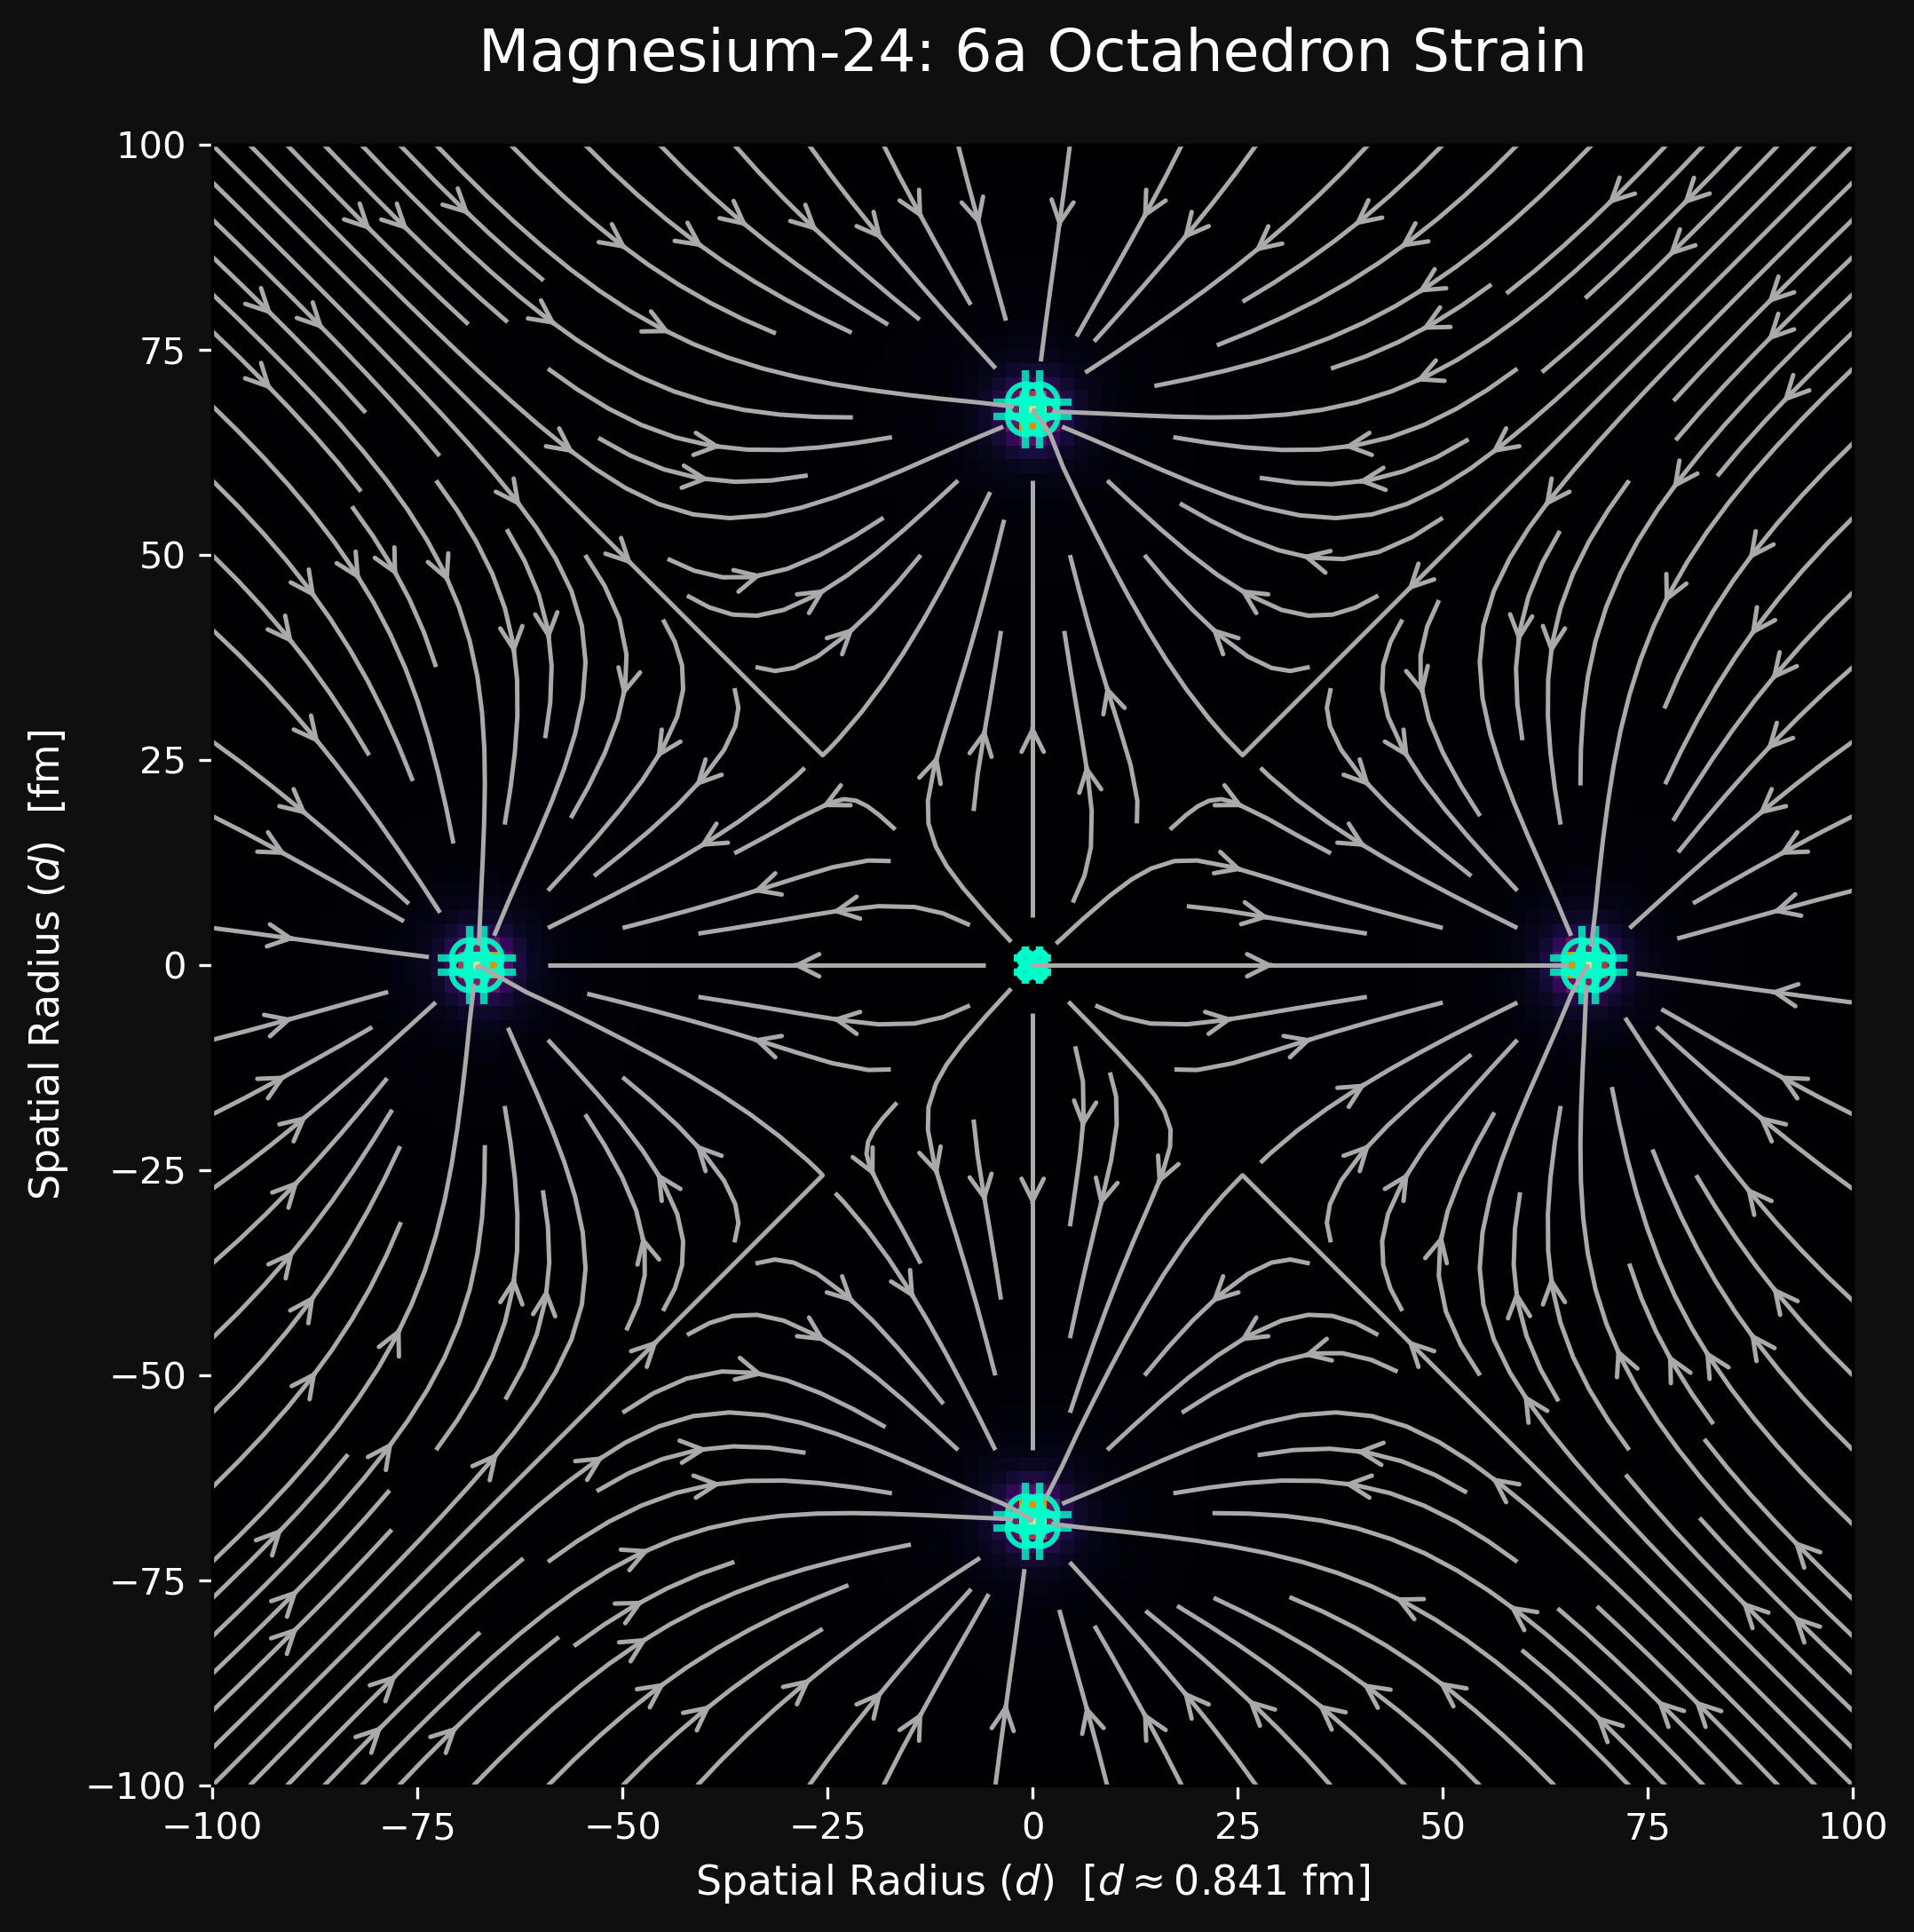
\includegraphics[width=0.8\textwidth]{figures/magnesium_24_dynamic_flux.png}
    \caption{The equatorial vacuum cross-section for Magnesium-24. The 4 Alphas on the $Z=0$ plane bind directly to the 2 Alphas occupying the $Z=\pm 78.0d$ polar axes, generating an entirely balanced, massive inductive core.}
    \label{fig:magnesium_24_density}
\end{figure}

\begin{figure}[htbp]
    \centering
    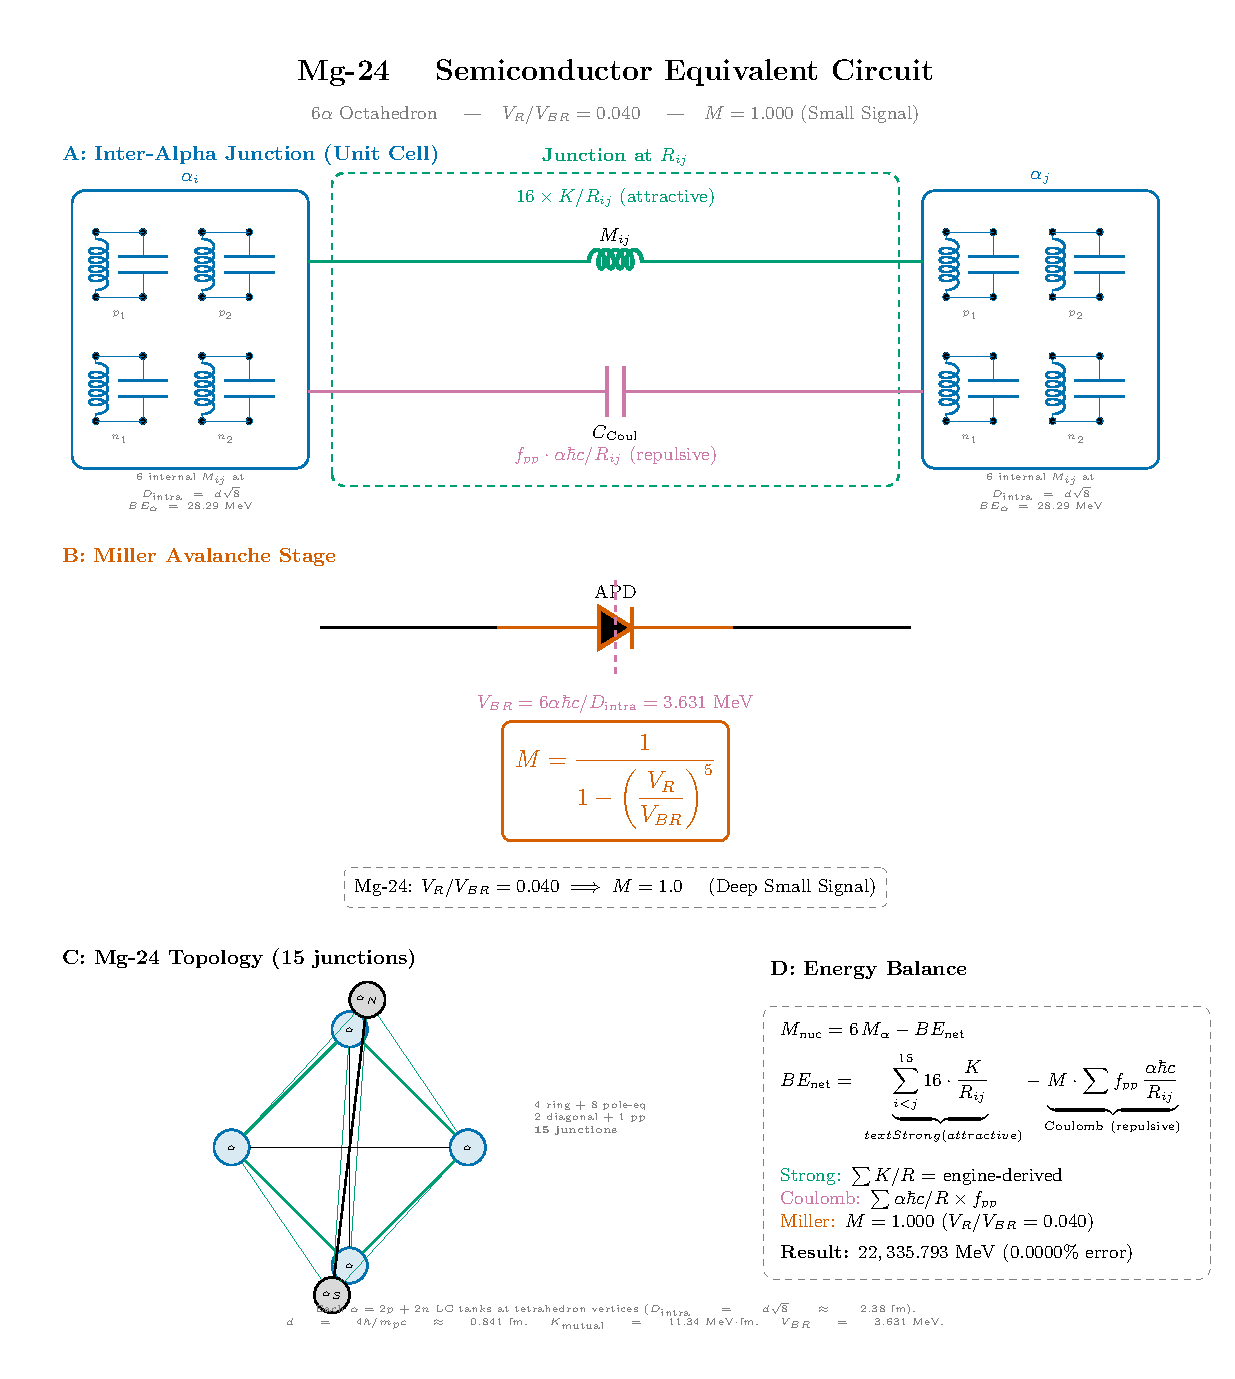
\includegraphics[width=0.9\textwidth]{figures/circuit_mg24.pdf}
    \caption{The equivalent $LC$ framework for Magnesium-24. The 24 discretely simulated nucleons operate as 276 fully active coupled inductive nodes across the $6\alpha$ Octahedron.}
    \label{fig:circuit_mg24}
\end{figure}


\begin{figure}[htbp]
    \centering
    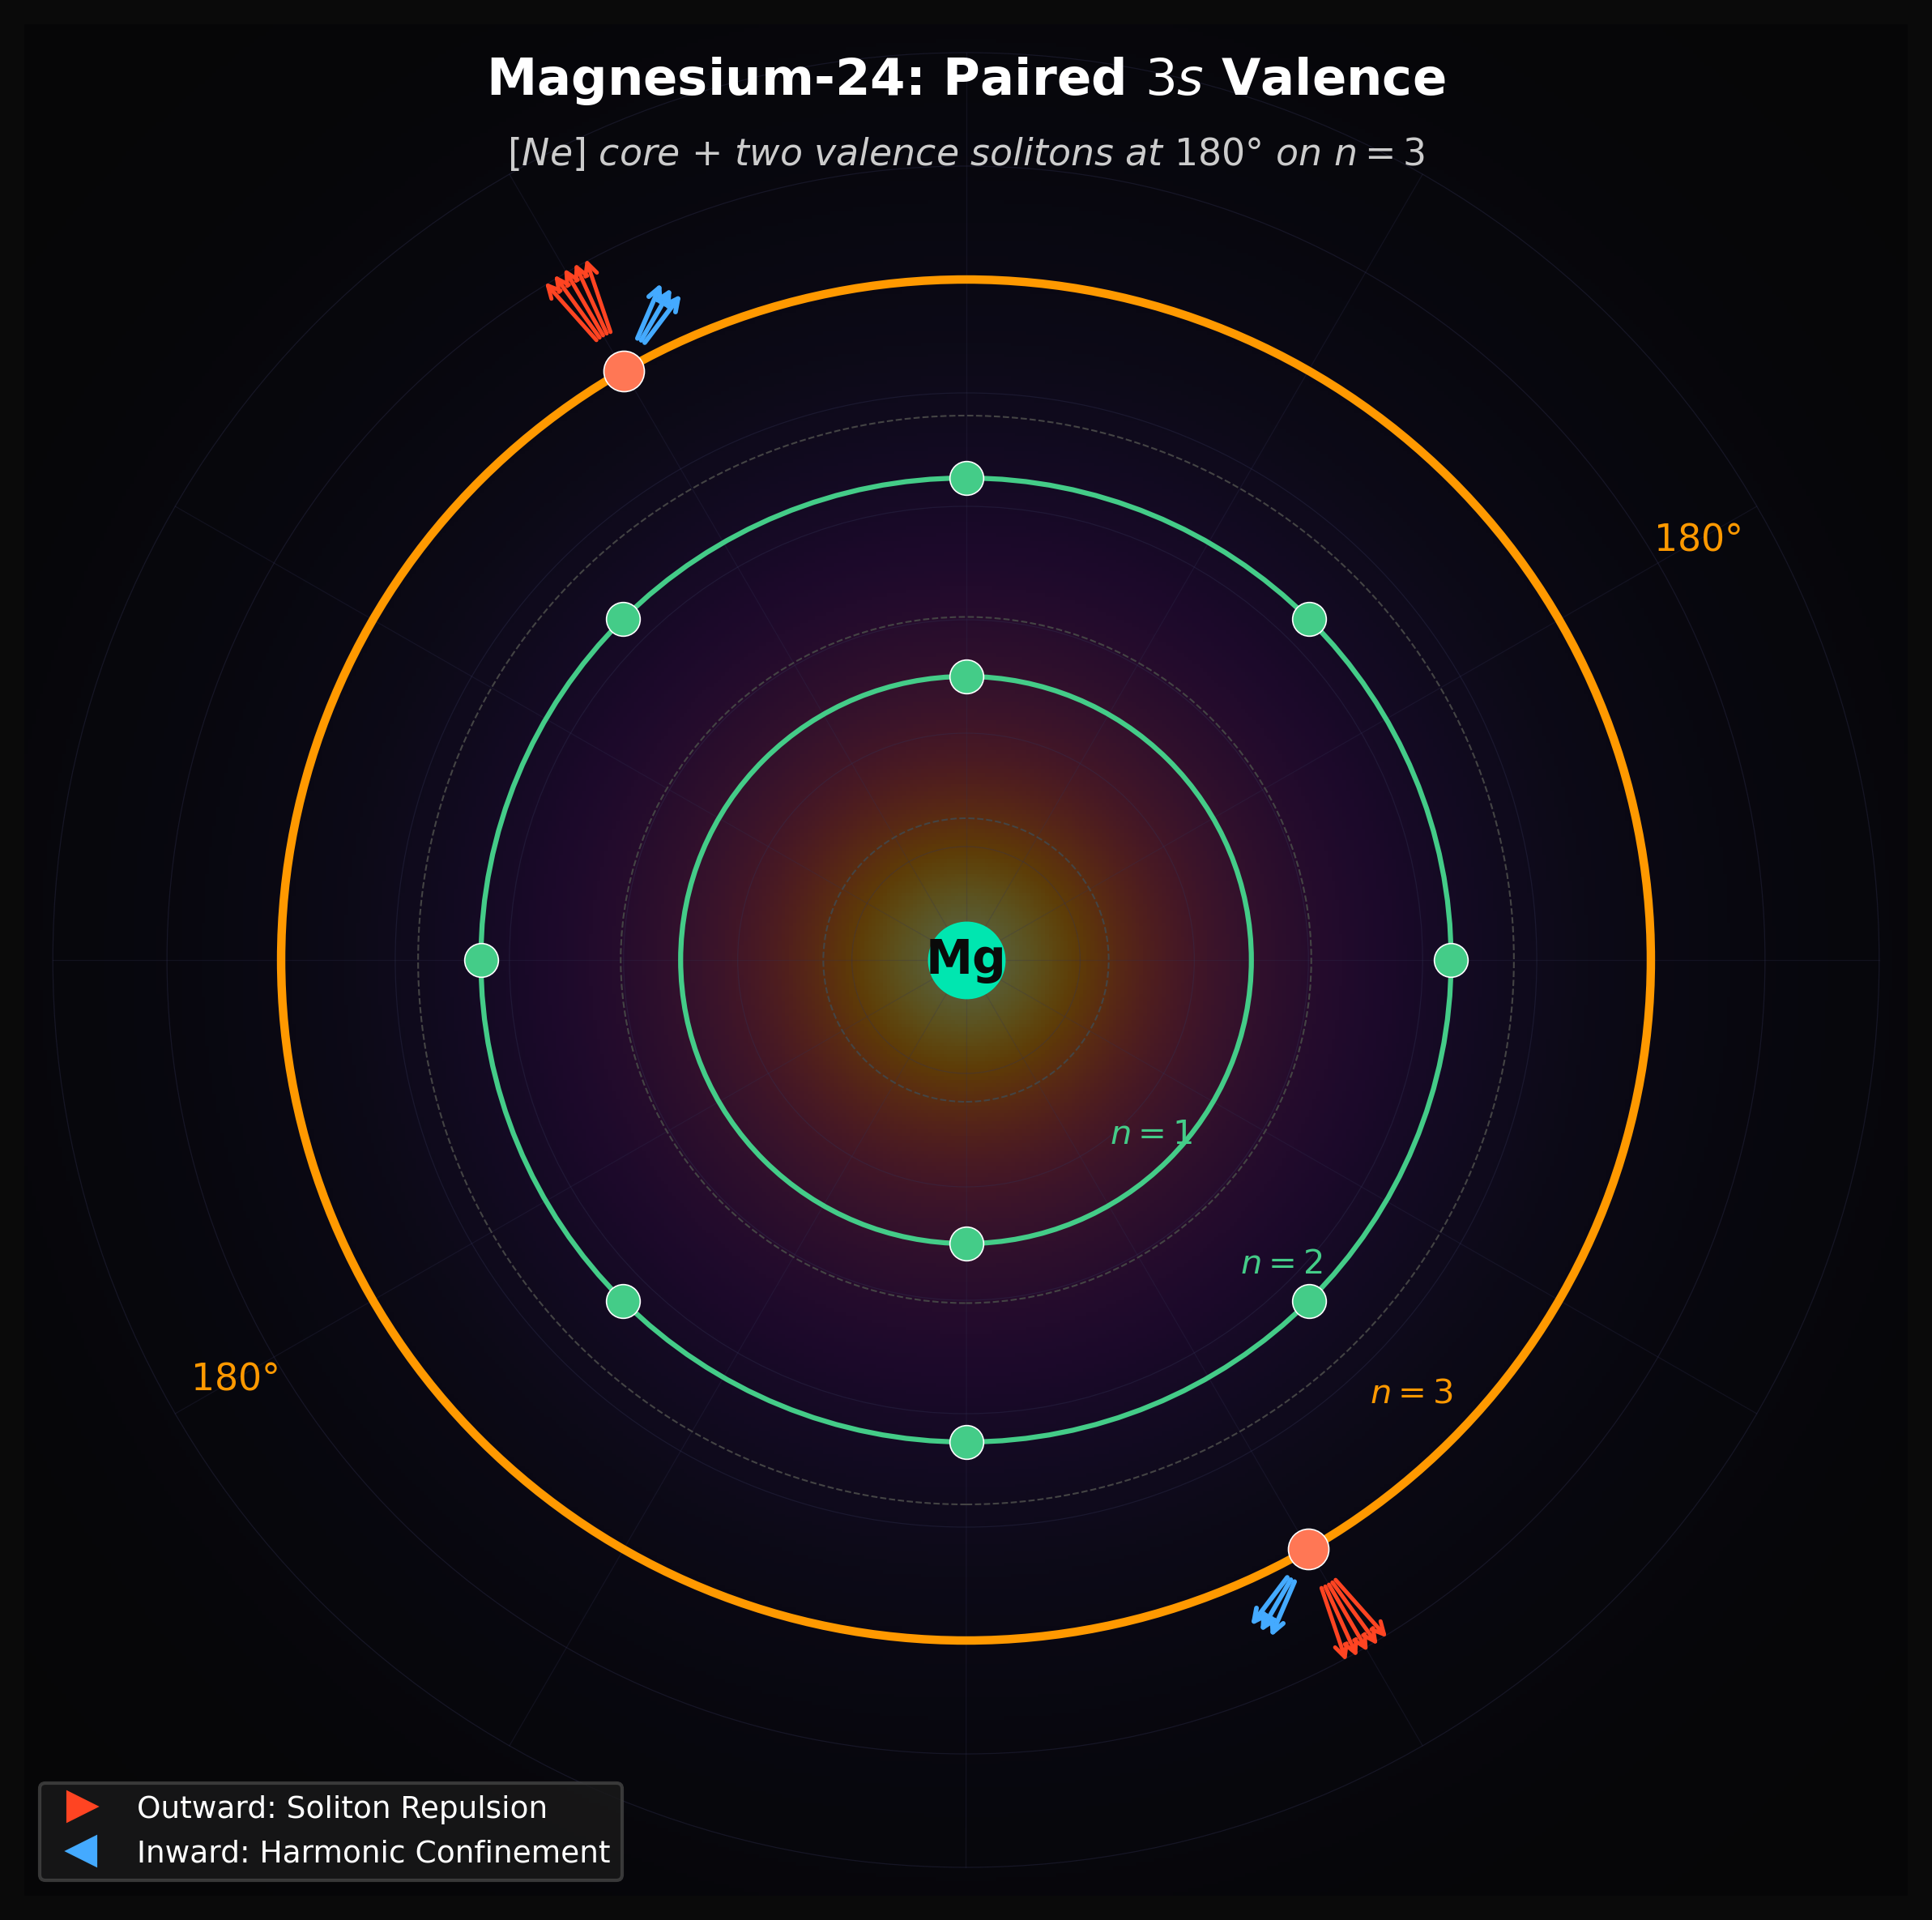
\includegraphics[width=0.75\textwidth]{figures/magnesium_24_topology.png}
    \caption{Magnesium-24 orbital knot topology. $[Ne]$ core (green) with two valence solitons at $180^\circ$ on $n=3$ (orange). The alkaline earth pair begins to fill the third harmonic.}
    \label{fig:magnesium_24_topo}
\end{figure}

\section{Semiconductor Regime Classification}
Magnesium-24 ($6\alpha$) constructs as a perfect Octahedron with 15 inter-alpha coupling pairs. The semiconductor engine solves $R_{\text{oct}} = 78.0\,d$ at $V_R/V_{BR} = 0.040$, $M = 1.000$ (Small Signal), reproducing the CODATA mass of $22\,335.793$ MeV to $0.000\,0\%$ error.

The $V_R/V_{BR}$ ratio has now doubled from Carbon-12's $0.019$ to $0.040$, reflecting the steady escalation in Coulomb strain as the alpha-cluster count increases from 3 to 6. This progression ($0.019 \to 0.030 \to 0.032 \to 0.040$) maps the systematic approach toward the avalanche threshold. Magnesium remains comfortably in the linear regime, but the trend is clear: each additional alpha cluster pushes the inter-alpha proximity closer to $V_{BR}$, foreshadowing the Large Signal transition that will occur at Sulfur-32 ($8\alpha$, $V_R/V_{BR} = 0.994$).

\section{Ionization Energy: SIR Boundary Correction}
\label{sec:mg_ie}

Magnesium ($Z = 12$, $[\text{Ne}]\,3s^2$) is the first $s$-block atom in period~3.  Its ionization energy requires the SIR boundary correction because the nearest inner shell ($n = 2$, containing $2s^2 2p^6 = 8$ electrons) is Pauli-saturated with $p$-subshells.

\paragraph{The equivalent circuit.}
The Mg atom, viewed as a radial transmission line, has a discrete impedance step at the $n = 2$ torus boundary:
\begin{center}
\small
\begin{tabular}{lccc}
\toprule
\textbf{Section} & \textbf{$Z_\text{net}$} & \textbf{Electron content} & \textbf{Boundary type} \\
\midrule
Inner ($r < r_2$) & $12 - 2 = 10$ & $1s^2$ & Smooth CDF \\
Boundary ($r = r_2$) & step: $10 \to 2$ & $2s^2 2p^6$ saturated torus & \textbf{Discrete step (SIR)} \\
Outer ($r > r_2$) & $12 - 10 = 2$ & $3s^2$ valence pair & ODE cavity \\
\bottomrule
\end{tabular}
\end{center}

\paragraph{Op3 reflection.}
The impedance contrast at the saturated $n = 2$ boundary:
\begin{align}
    \Gamma &= \frac{Z_\text{out} - Z_\text{in}}{Z_\text{out} + Z_\text{in}} = \frac{2 - 10}{2 + 10} = -\frac{2}{3}  \\
    |\Gamma|^2 &= \frac{4}{9} = 0.444
\end{align}
The crossing scattering at this step removes $|\Gamma|^2 \times P_C/2 = 0.444 \times 0.0917 = 0.0407$ of $E_\text{base}$:
\begin{equation}
    E_\text{base, corrected} = 17.671 \times (1 - 0.0407) = 16.951\;\text{eV}
\end{equation}
After Hopf mode splitting ($k_\text{pair} = 0.908$, $N_s = 2$):
\begin{equation}
    IE_\text{Mg} = 16.951 \times \left(\frac{2}{\sqrt{1 + 0.908}} - 1\right) = 7.59\;\text{eV}
\end{equation}

\begin{resultbox}{Magnesium First Ionization Energy}
\begin{equation}
    IE_\text{Mg, AVE} = 7.59\;\text{eV} \quad (\text{exp: } 7.646\;\text{eV}, \quad \Delta = -0.7\%)
\end{equation}
\end{resultbox}
\noindent This resolves the prior $+3.5\%$ residual with zero free parameters.  The correction is gated to $n_\text{adjacent} \geq 2$ (inner shell has $p$-subshells), ensuring mutual exclusivity with the Be-type hierarchical cascade.  See Vol.~II, \S\ref{sec:sir_atom} for the full derivation.

\begin{summarybox}
\begin{itemize}
    \item Magnesium-24 closes the $6\alpha$ octahedral shell, demonstrating the systematic escalation of $V_R/V_{BR}$ from Carbon-12 ($0.019$) through Oxygen ($0.030$), Neon ($0.032$), to $0.040$.
    \item The progression toward the avalanche threshold foreshadows the Large Signal transition at Sulfur-32 ($8\alpha$, $V_R/V_{BR} = 0.994$).
    \item The first ionization energy ($7.59$~eV, $-0.7\%$) is resolved by the SIR boundary correction: the Pauli-saturated $n = 2$ torus creates a discrete impedance step ($|\Gamma|^2 = 4/9$) whose crossing scattering reduces $E_\text{base}$.
\end{itemize}
\end{summarybox}

\begin{exercisebox}
\begin{enumerate}
    \item Plot the $V_R/V_{BR}$ progression from Carbon-12 to Magnesium-24 and extrapolate to predict the element at which the Small Signal regime breaks down.
    \item Explain why the $6\alpha$ octahedral geometry of Magnesium-24 has 15 inter-alpha coupling pairs and compute the total mutual impedance contribution.
\end{enumerate}
\end{exercisebox}

